\documentclass{standalone}
\usepackage{amsmath}
\usepackage{amssymb}
\usepackage{warpcol}
\usepackage{array}
\usepackage{esint}
\usepackage{subfig}
\usepackage{rotating}
\usepackage{booktabs}
\usepackage{paralist}
\usepackage{graphicx}
\usepackage{physics}
\usepackage{ucs}
\usepackage{indentfirst}
\usepackage{tikz}
\usepackage{colortbl}
\usepackage{xcolor}
\usepackage{xeCJK}
    \setCJKmainfont[BoldFont={Noto Serif CJK SC Bold},ItalicFont={FangSong}]{Noto Serif CJK SC}
    \setCJKsansfont[BoldFont={Noto Sans CJK SC Bold},ItalicFont={KaiTi}]{Noto Sans CJK SC}
    \setCJKmonofont[BoldFont={Noto Sans Mono CJK SC Bold}]{Noto Sans Mono CJK SC}

\DeclareUnicodeCharacter{"00B0}{\textdegree}
\DeclareUnicodeCharacter{"2103}{\textcelsius}

\pgfsetxvec{\pgfpoint{2em}{0}}
\pgfsetyvec{\pgfpoint{0}{2em}}

\usetikzlibrary{angles,patterns,datavisualization,plotmarks,arrows.meta,datavisualization.formats.functions,decorations.markings}

\begin{document}
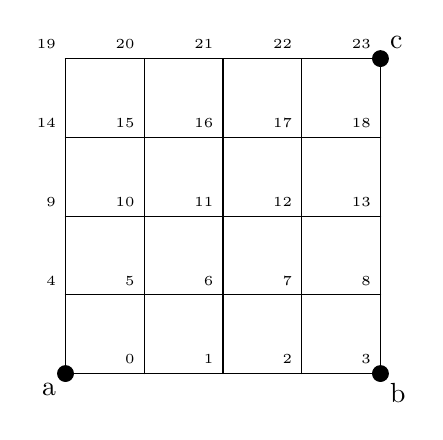
\begin{tikzpicture}
\foreach \x in {-2,-1,...,2}{
    \draw[line cap=round] (-2, \x) -- (2, \x);
    \draw[line cap=round] (\x, -2) -- (\x, 2);
}
\foreach \y [count=\yi] in {-1,0,...,2}{
    \foreach \x [count=\xi,evaluate={\xi,\yi} as \idx using {\yi*5+\xi-2}] in {-2,-1,...,2}{
        \node[anchor=south east] at (\x, \y) {\pgfmathparse{int(\idx)}\tiny\pgfmathresult};
    }
}
\foreach \idx[evaluate=\idx as \x using \idx-1] in {0,1,2,3}{
    \node[anchor=south east] at (\x, -2) {\tiny\idx};
}
\filldraw (-2, -2) node[below left] {a} circle (0.1);
\filldraw (2, -2) node[below right] {b} circle (0.1);
\filldraw (2, 2) node[above right] {c} circle (0.1);
\end{tikzpicture}
\end{document}
